

\chapter{Estudo de retas}\label{cap_er}
\thispagestyle{fancy}

Neste capítulo, vamos estudar retas no espaço (euclidiano) tridimensional. Salvo explicitado diferente, iremos trabalhar sobre o sistema de coordenadas canônico, i.e. um sistema de coordenadas ortonormal (veja Seção \ref{cap_scoord_sec_scoord}).

\section{Equações da reta}\label{cap_ert_sec_eqsreta}

Nesta seção, vamos desenvolver equações para a representação de retas no espaço tridimensional.

\begin{figure}[H]
  \centering
  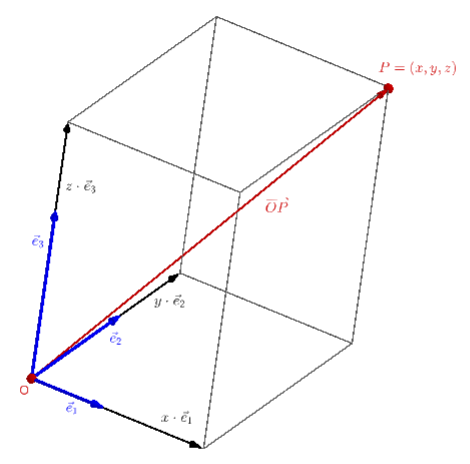
\includegraphics[width=0.8\textwidth]{cap_er/dados/fig_er_ilu0/fig}
  \caption{Ilustração de uma reta $r$ em um sistema de coordenadas ortonormal.}
\end{figure}

\subsection{Equação vetorial de uma reta}

Seja $r$ uma reta dada, $\vec{v}$ um vetor paralelo a $r$ e $A$ um ponto de $r$ (veja a Figura~\ref{fig:er_vet}). Assim sendo, $P=(x,y,z)$ é um ponto de $r$ se, e somente se, o vetor $\overrightarrow{AP}$ tem a mesma direção de $\vec{v}$. i.e. existe $\lambda\in\mathbb{R}$ tal que
\begin{equation}
  {\color{blue}\overrightarrow{AP} = \lambda\vec{v}}.
\end{equation}
Esta é chamada \emph{equação vetorial da reta} $r$.

\begin{figure}[H]
  \centering
  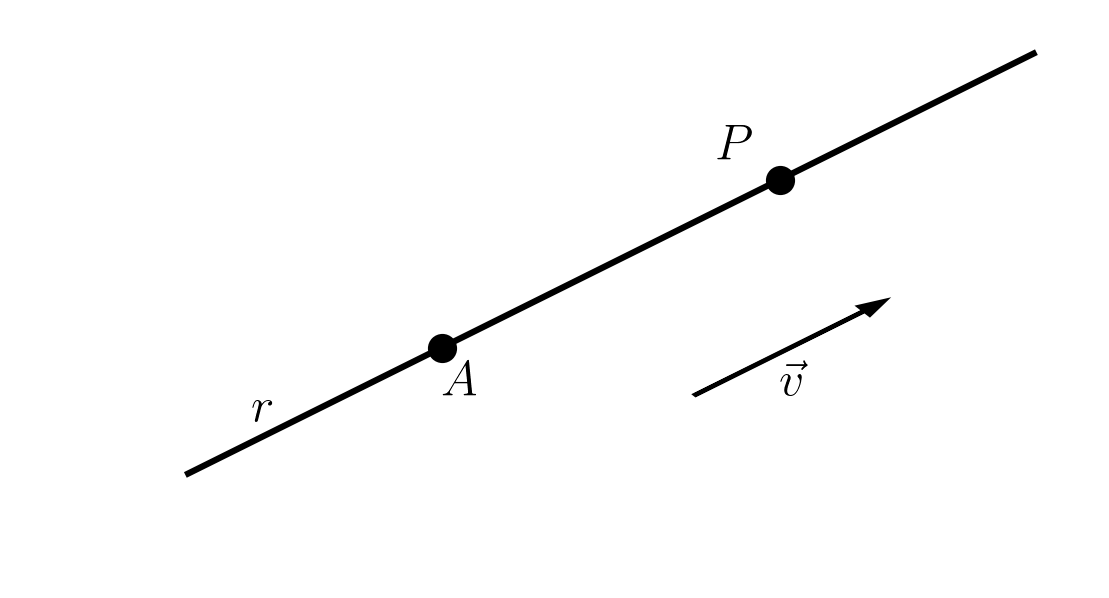
\includegraphics[width=0.5\textwidth]{./cap_er/dados/fig_er_vet/fig_er_vet}
  \caption{Equação vetorial de uma reta.}
  \label{fig:er_vet}
\end{figure}

Observe que para obtermos uma equação vetorial de uma dada reta, podemos escolher qualquer ponto $A\in r$ e qualquer vetor $\vec{v}\parallel r$, $\vec{v}\neq\vec{0}$. O vetor $\vec{v}$ escolhido é chamado de \emph{vetor diretor}.

\begin{ex}\label{ex:er_vet}
  Seja $r$ a reta que passa pelos pontos $A=(-1,-1,-2)$ e $B = (2,1,3)$ (veja a Figura \ref{fig:ex_er_vet}). O vetor
  \begin{equation}
    \vec{v} = \overrightarrow{AB} = (2-(-1),1-(-1),3-(-2)) = (3,2,5)
  \end{equation}
  é um vetor diretor de $r$. Desta forma, uma equação vetorial da reta $r$ é
  \begin{equation}
    \overrightarrow{AP} = \lambda\vec{v}.
  \end{equation}
  \begin{figure}[H]
    \centering
    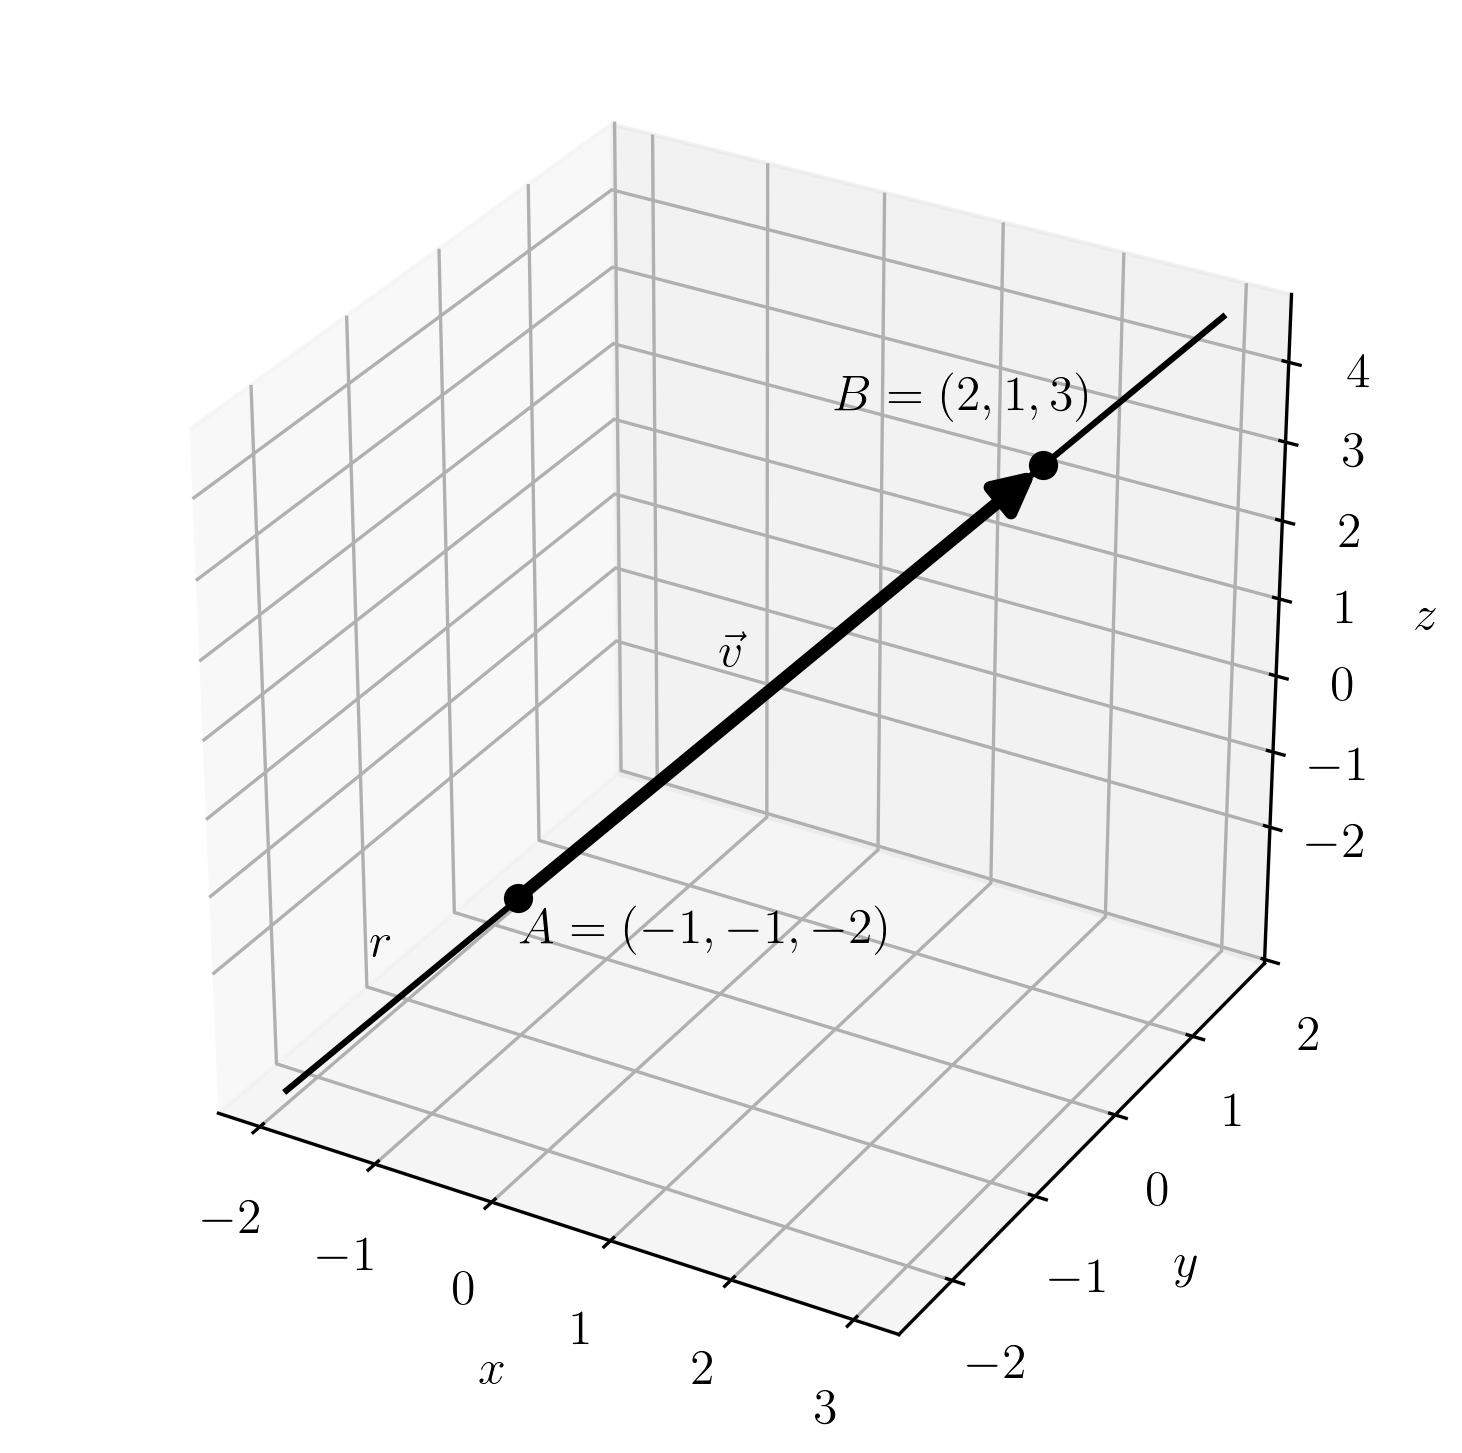
\includegraphics[width=0.7\textwidth]{./cap_er/dados/fig_ex_er_vet/fig_ex_er_vet}
    \caption{Esboço da reta discutida no Exemplo \ref{ex:er_vet}.}
    \label{fig:ex_er_vet}
  \end{figure}  
\end{ex}

\subsection{Equações paramétricas de uma reta}

Seja $r$ uma reta que passa pelo ponto $A = (x_A,y_A,z_A)$ e tenha vetor diretor $\vec{v} = (v_1,v_2,v_3)$. Da equação vetorial, temos que $P = (x,y,z)\in r$ se, e somente se, existe $\lambda\in\mathbb{R}$ tal que
\begin{equation}
  \overrightarrow{AP} = \lambda\vec{v}.
\end{equation}
Equivalentemente,
\begin{equation}
  \underbrace{(x-x_A,y-y_A,z-z_A)}_{\overrightarrow{AP}} = \lambda \underbrace{(v_1,v_2,v_3)}_{\vec{v}}.
\end{equation}
Então,
\begin{align}
  x-x_A &= \lambda v_1,\\
  y-y_A &= \lambda v_2,\\
  z-z_A &= \lambda v_3,
\end{align}
donde
\begin{align}
  {\color{blue}x} &{\color{blue}= x_A + \lambda v_1},\\
  {\color{blue}y} &{\color{blue}= y_A + \lambda v_2},\\
  {\color{blue}z} &{\color{blue}= z_A + \lambda v_3},
\end{align}
as quais são chamadas de \emph{equações paramétricas} da reta $r$.

\begin{ex}\label{ex:ex_er_par}
  A reta $r$ discutida no Exemplo \ref{ex:er_vet} tem equações paramétricas
  \begin{align}
    x &= -1 + 3\lambda,\\
    y &= -1 + 2\lambda,\\
    z &= -2 + 5\lambda.
  \end{align}
  De fato, tomando $\lambda = 0$, temos $(x,y,z) = (-1,-1,-2) = A\in r$. E, tomado $\lambda = 1$, temos $(x,y,z) = (-1+3,-1+2,-2+5) = (2,1,3) = B\in r$. Ou seja, as equações paramétricas acima representam a reta que passa pelos pontos $A$ e $B$.

  \ifispython
  Com o \verb+Sympy+, podemos plotar o gráfico de $r$ usando o seguinte código:
\begin{verbatim}
var('lbda',real=True)
plot3d_parametric_line(-1+3*lbda,-1+2*lbda,-2+5*lbda,(lbda,-1,2))
\end{verbatim}
  \fi
\end{ex}

\subsection{Equações da reta na forma simétrica}

Seja $r$ uma reta que passa pelo ponto $A = (x_A,y_A,z_A)$ e tem $\vec{v} = (v_1,v_2,v_3)$ como vetor diretor. Então, $r$ tem as equações paramétricas
\begin{align}
  x &= x_A + v_1\lambda,\\
  y &= y_A + v_2\lambda,\\
  z &= z_A + v_3\lambda.
\end{align}
Isolando $\lambda$ em cada uma das equações, obtemos
\begin{align}
  \lambda &= \frac{x-x_A}{v_1},\\
  \lambda &= \frac{y-y_A}{v_2},\\
  \lambda &= \frac{z-z_A}{v_3}.
\end{align}
Daí, temos
\begin{equation}
  {\color{blue}\frac{x-x_A}{v_1} = \frac{y-y_A}{v_2} = \frac{z-z_A}{v_3}},
\end{equation}
as quais são as \emph{equações da reta na forma simétrica}.

\begin{ex}
  No Exemplo \ref{ex:ex_er_par}, consideramos a reta $r$ de equações paramétricas
  \begin{align}
    x &= -1 + 3\lambda,\\
    y &= -1 + 2\lambda,\\
    z &= -2 + 5\lambda.    
  \end{align}
  Para obtermos as equações de $r$ na forma simétrica, basta isolarmos $\lambda$ em cada equação. Com isso, obtemos
  \begin{equation}
    \frac{x+1}{3} = \frac{y+1}{2} = \frac{z+2}{5}.
  \end{equation}
\end{ex}

\subsection*{Exercícios resolvidos}

\begin{exeresol}
  Seja $r$ a reta que passa pelo ponto $A = (-1,-1,-2)$ e tem $\vec{v} = (3,2,5)$ como vetor diretor. Determine o valor de $x$ de forma que $P = \left(x, 0, \frac{1}{2}\right)$ seja um ponto de $r$.
\end{exeresol}
\begin{resol}
  Da equação vetorial da reta $r$, temos que $P = \left(x,0,\frac{1}{2}\right)$ é um ponto de $r$ se, e somente se, existe $\lambda\in\mathbb{R}$ tal que
  \begin{equation}
    \overrightarrow{AP} = \lambda\vec{v}.
  \end{equation}
  Ou seja,
  \begin{equation}
    \left(x-(-1),0-(-1),\frac{1}{2}-(-2)\right) = \lambda (3,2,5).
  \end{equation}
  Ou, equivalentemente,
  \begin{equation}
    \left(x+1,1,\frac{5}{2}\right) = \lambda (3,2,5).
  \end{equation}
  Usando a segunda coordenada destes vetores, temos
  \begin{gather}
    1 = \lambda\cdot 2\\
    \lambda = \frac{1}{2}.
  \end{gather}
  Assim, da primeira coordenada dos vetores, temos
  \begin{gather}
    x+1 = \lambda\cdot 3 \\
    x+1 = \frac{1}{2}\cdot 3\\
    x = \frac{3}{2}-1\\
    x= \frac{1}{2}.
  \end{gather}
\end{resol}

\begin{exeresol}
  Seja $r$ a reta de equações paramétricas
  \begin{align}
    x &= 1 -\lambda,\\
    y &= \lambda,\\
    z &= -3.
  \end{align}
  Determine uma equação vetorial de $r$.
\end{exeresol}
\begin{resol}
  Nas equações paramétricas de uma reta, temos que os coeficientes constantes estão associados a um ponto da reta. Os coeficientes do parâmetro $\lambda$ estão associados a um vetor diretor. Assim sendo, das equações paramétricas da reta $r$, temos que
  \begin{equation}
    A = (1,0,-3)\in r
  \end{equation}
  e
  \begin{equation}
    \vec{v} = (-1,1,0)
  \end{equation}
  é um vetor diretor. Logo, temos que a reta $r$ tem equação vetorial
  \begin{equation}
    \overrightarrow{AP} = \lambda\vec{v},
  \end{equation}
  com $A = (1,0,3)$ e $\vec{v} = (-1,1,0)$.
\end{resol}

\begin{exeresol}
  Sabendo que $r$ é uma reta que passa pelos pontos $A = (2,-3,1)$ e $B = (-1,1,0)$, determine o valor de $t$ tal que
  \begin{align}
    x &= 2 + t\lambda,\\
    y &= -2 + 4\lambda,\\
    z &= 1 -\lambda,
  \end{align}
  sejam equações paramétricas de $r$.
\end{exeresol}
\begin{resol}
  Para que estas sejam equações paramétricas de $r$, é necessário que $\vec{v} = (t,4,-1)$ seja um vetor diretor de $r$. Em particular, $\vec{v} \parallel \overrightarrow{AB}$. Logo, existe $\beta\in\mathbb{R}$ tal que
  \begin{gather}
    \vec{v} = \beta\overrightarrow{AB}\\
    (t,4,-1) = \beta (-1-2,1-(-3),0-1) \\
    (t,4,-1) = \beta (-3,4,-1).
  \end{gather}
  Das segunda e terceira coordenadas, temos $\beta = 1$. Daí, comparando pela primeira coordenada, temos
  \begin{gather}
    t = -3\beta\\
    t = -3.
  \end{gather}
\end{resol}

\begin{exeresol}\label{exeresol:er_sim}
  Seja $r$ uma reta de equações na forma simétrica
  \begin{equation}
    \frac{x+1}{2} = \frac{y-2}{3} = \frac{1-z}{2}.
  \end{equation}
  Determine equações paramétricas para esta reta e faça um esboço de seu gráfico.
\end{exeresol}
\begin{resol}
  Podemos obter equações paramétricas desta reta a partir de suas equações na forma simétrica. Para tanto, basta tomar o parâmetro $\lambda$ tal que
  \begin{align}
    \lambda &= \frac{x+1}{2},\\
    \lambda &= \frac{y-2}{3},\\
    \lambda &= \frac{1-z}{2}.
  \end{align}
  Daí, isolando $x$, $y$ e $z$ em cada uma destas equações, obtemos
  \begin{align}
    x &= -1 + 2\lambda,\\
    y &= 2 + 3\lambda,\\
    z &= 1 - 2\lambda.
  \end{align}
  Para fazermos um esboço do gráfico desta reta, basta traçarmos a reta que passa por dois de seus pontos. Por exemplo, tomando $\lambda = 0$, temos $A = (-1,2,1)\in r$. Agora, tomando $\lambda = 1$, temos $B = (1,5,-1)\in r$. Desta forma, obtemos o esboço dado na Figura \ref{fig:exeresol_er_sim}.

  \begin{figure}[H]
    \centering
    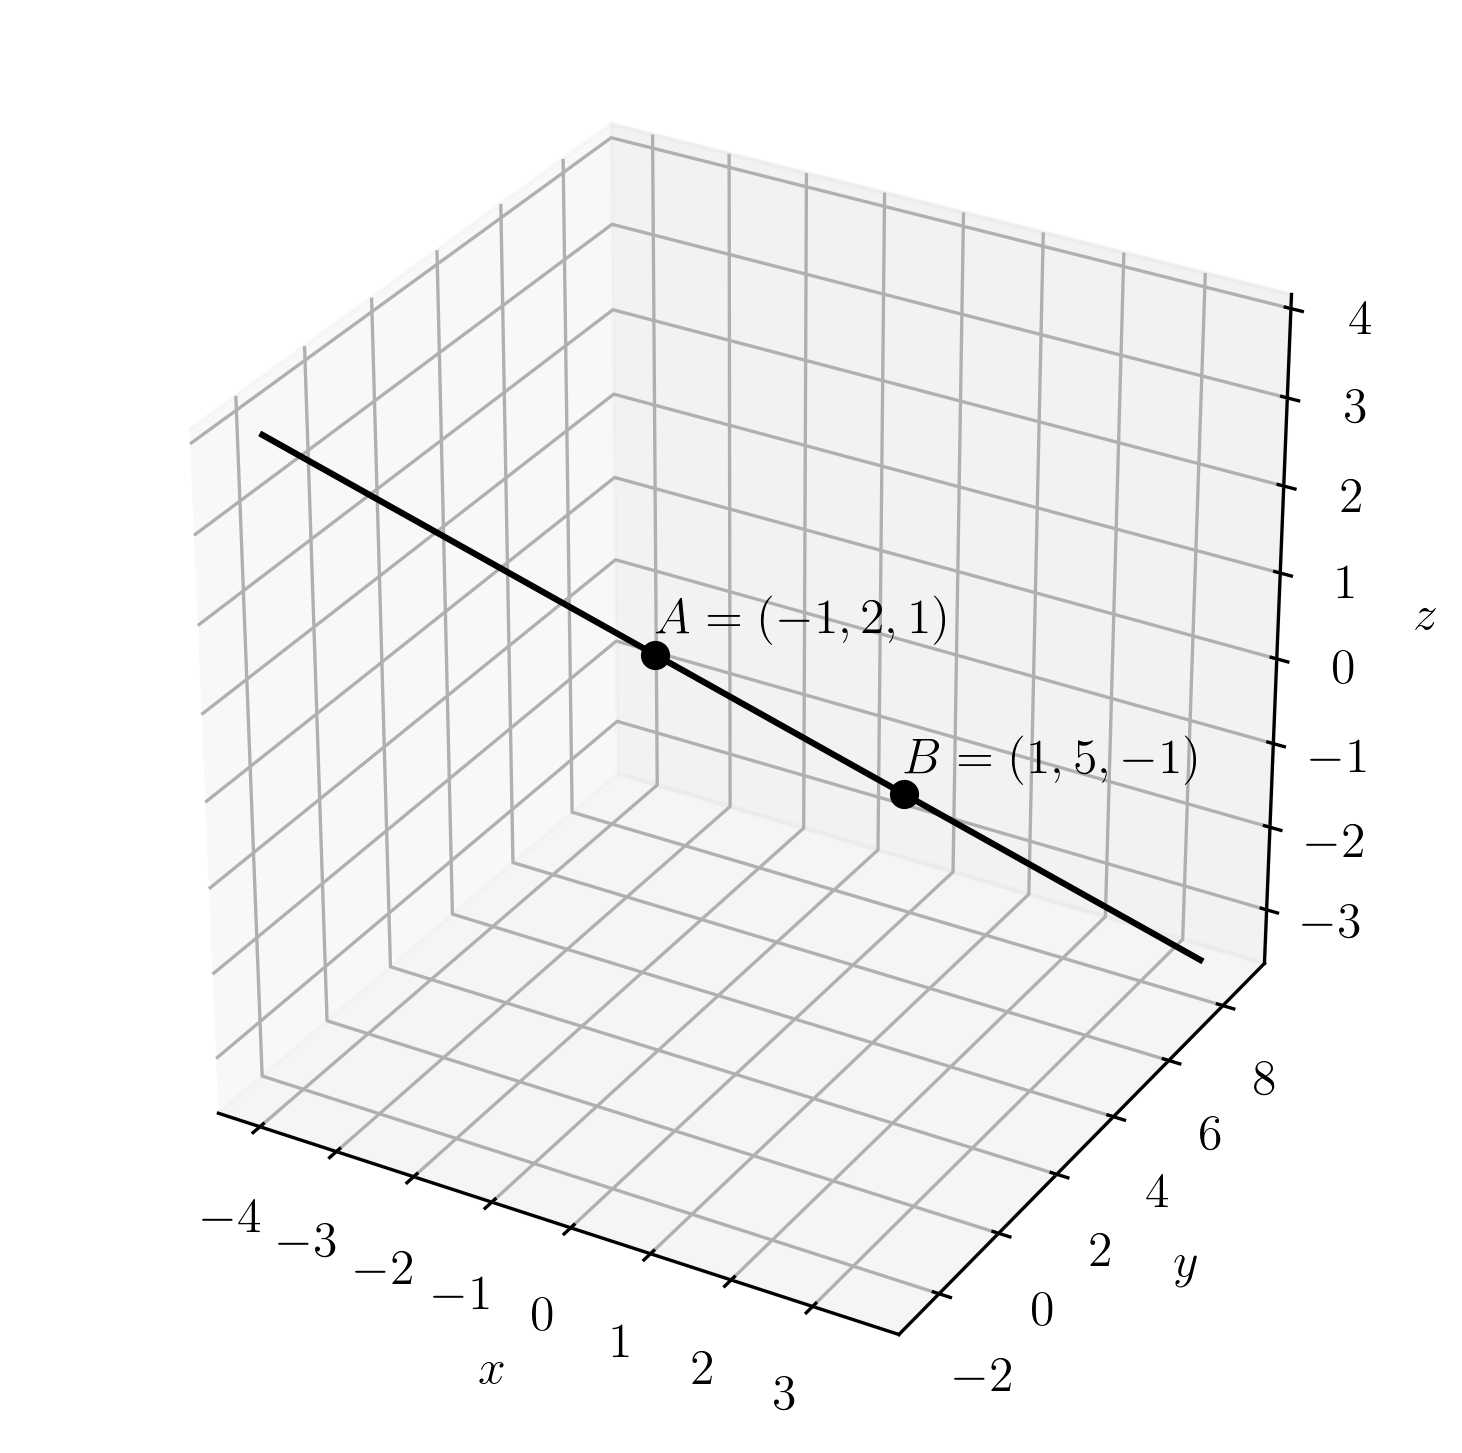
\includegraphics[width=0.7\textwidth]{./cap_er/dados/fig_exeresol_er_sim/fig_exeresol_er_sim}
    \caption{Esboço do gráfico da reta $r$ do Exercício Resolvido \ref{exeresol:er_sim}.}
    \label{fig:exeresol_er_sim}
  \end{figure}
\end{resol}

\subsection*{Exercícios}

\begin{exer}
  Seja a reta que passa pelos pontos $A=(1,-2,0)$ e $B=(-1,-1,1)$. Determine:
  \begin{enumerate}[a)]
  \item sua equação vetorial.
  \item suas equações paramétricas.
  \item suas equações na forma simétrica.
  \end{enumerate}
\end{exer}
\begin{resp}
  a) $\overrightarrow{AP}=\lambda\vec{v}$, $\vec{v}=(-2,1,1)$; b) $x=1-2\lambda$, $y=-2+\lambda$, $z=\lambda$; c) $\frac{x-1}{-2}=y+2=z$
\end{resp}

\begin{exer}
  Seja a reta que passa pelo ponto $A=(0,1,-1)$ e tem vetor diretor $\vec{v}=(2,-1,1)$. Determine $x$ tal que $B=(1,x,-\frac{1}{2})$.
\end{exer}
\begin{resp}
  $x=\frac{1}{2}$
\end{resp}

\begin{exer}
  Considere a reta de equações na forma simétrica
  \begin{equation}
    \frac{x-1}{-2}=\frac{y+1}{3}=z-1.
  \end{equation}
  Encontre um ponto e um vetor diretor desta reta.
\end{exer}
\begin{resp}
  $A=(1,-1,1)$, $\vec{v}=(-2,3,1)$
\end{resp}

\begin{exer}
  Seja a reta $r$ de equações paramétricas
  \begin{align}
    x &= \lambda\\
    y &= 2-\lambda\\
    z &= -1+\lambda
  \end{align}
  Determine as equações na forma simétrica da reta que passa pelo ponto $A=(1,-1,0)$ e é paralela a reta $r$.
\end{exer}
\begin{resp}
  $x-1=\frac{y+1}{-1}=z$
\end{resp}

\begin{exer}
  Seja a reta $r$ de equações paramétricas
  \begin{align}
    x &= \lambda\\
    y &= 2-\lambda\\
    z &= -1+\lambda
  \end{align}
  Determine as equações paramétricas da reta que passa pelo ponto $A=(1,-1,0)$ e é perpendicular a reta $r$.
\end{exer}
\begin{resp}
  $x=1-\lambda$, $y=-1-2\lambda$, $z=-\lambda$
\end{resp}
